\section{Discussion}
The discussion section aims at interpreting the results in light of the project's objectives.
The most important goal of this section is to interpret the results so that the reader is informed of the insight or answers that the results provide.
This section should also present an evaluation of the particular approach taken by the group.
For example: Based on the results, how could the experimental procedure be improved?
What additional, future work may be warranted?
What recommendations can be drawn?


\begin{figure}[ht]
\centering
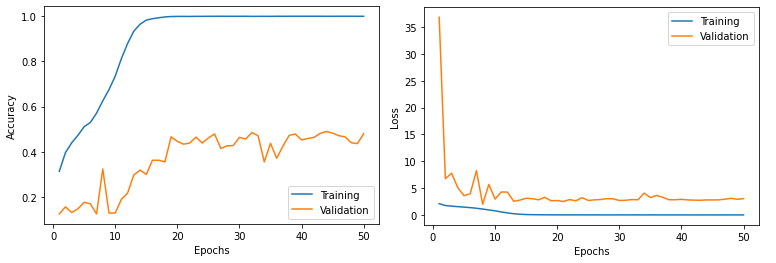
\includegraphics[scale=0.6]{images/2021-val-train.png}
\caption{Accuracy and Loss function of the training and validation set.}
\label{fig:GP_Acq}
\end{figure}


\begin{figure}[ht]
\centering
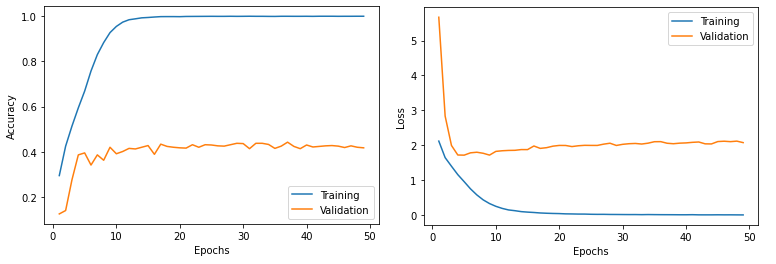
\includegraphics[scale=0.6]{images/tuned-val-train.png}
\caption{Accuracy and Loss function of the training and validation set.}
\label{fig:GP_Acq}
\end{figure}
